\begin{frame}
  \frametitle{Artificial Neural Networks}
  \begin{figure}
    \centering
    \resizebox{0.7\textwidth}{!}{\begin{neuralnetwork}[height=5]
  \tikzstyle{input neuron}=[neuron, draw, fill=white]
  \tikzstyle{hidden neuron}=[neuron, draw, fill=white]
  \tikzstyle{output neuron}=[neuron, draw, fill=white]
  \tikzstyle{link} = [->, shorten <=0pt, node distance=\nn@layerspacing, thin, draw=black];
  \inputlayer[count=4, bias=false, title=Input\\layer]
  \hiddenlayer[count=5, bias=false, title=Hidden\\layer] \linklayers
  \outputlayer[count=3, title=Output\\layer] \linklayers
\end{neuralnetwork}
}
    \caption{A common ANN-structure represented by a directed graph.}
  \end{figure}
\end{frame}

\begin{frame}
  \frametitle{Artificial Neural Networks}
  \begin{itemize}
    \item Class of machine learning algorithms
      \begin{itemize}
        \item Loosely inspired by biological nervous systems
      \end{itemize}
    \item Collection of artificial neurons that are connected with
      each other
      \begin{itemize}
        \item Enables them to exchange signals along their connections
        \item Can be represented by a directed graph
      \end{itemize}
    \item Usually arranged in layers
      \begin{itemize}
        \item \textit{Input Layer} collects input signals and passes
          them on
        \item \textit{Hidden Layers} apply transformations to incoming
          signals and pass the outcomes further into the network
        \item \textit{Output Layer} applies a final transformation
          representing the networks' result
      \end{itemize}
    \item Goal: Convert input into meaningful output by applying
      multiple transformations
  \end{itemize}
\end{frame}

\begin{frame}
  \frametitle{Modeling Artificial Neurons}
  \begin{figure}
    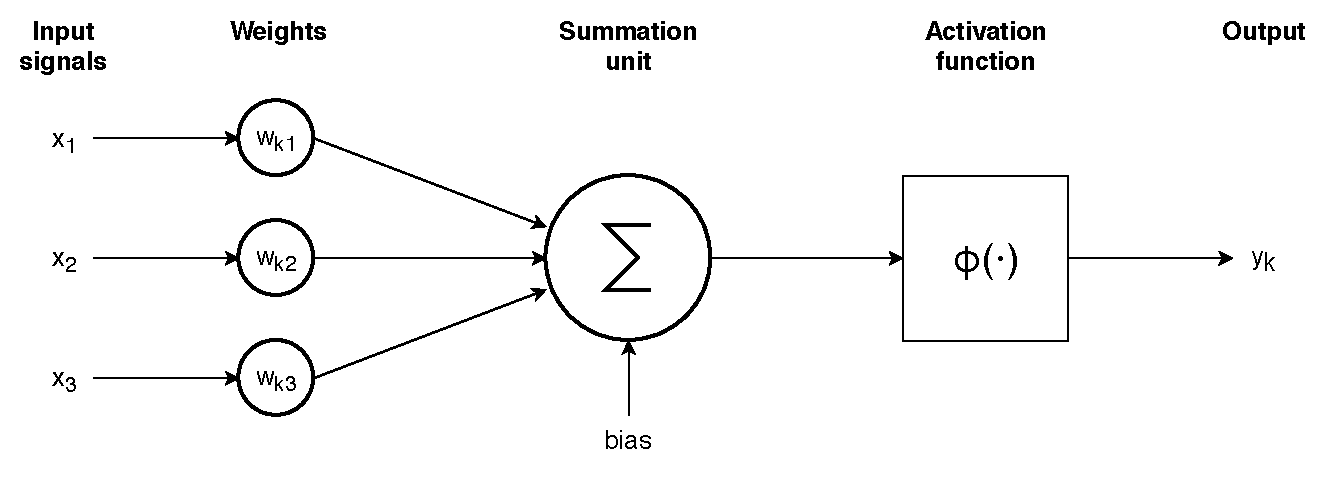
\includegraphics[width=.9\textwidth]{../figures/single_neuron}
    \caption{The components of a single artificial neuron \(k\).}
  \end{figure}
\end{frame}

\begin{frame}
  \frametitle{Components of the neural model}
  \begin{itemize}
   \item A set of weighted inputs
     \begin{itemize}
       \item Each input originating from neuron \(j\) and traveling
         into neuron \(k\) is first multiplied by a weight \(w_{kj}\)
     \end{itemize}
   \item A summation unit
     \begin{itemize}
       \item All the weighted inputs are summed and a constant value,
         the \textit{bias}, is added to yield the result \(z_k\)
     \end{itemize}
   \item An activation function
     \begin{itemize}
       \item Applies a non-linear transformation \(\phi(\cdot)\) to
         the output of the summation unit
       \item This result, called \(y_k\), is propagated further into
         the network alongside the connections
     \end{itemize}
  \end{itemize}
\end{frame}
